\section{Introduction}
\label{sec:intro}


In this laboratory assignement the objective is to study an amplifier together with some of its properties, namely the input and output impedances, the voltage gain and also the influence of the frequency on this gain. The specific circuit used in the Octave and Ngspice software is the one illustrated:


\begin{figure} [!htb] 
  \minipage{0.9\textwidth}
  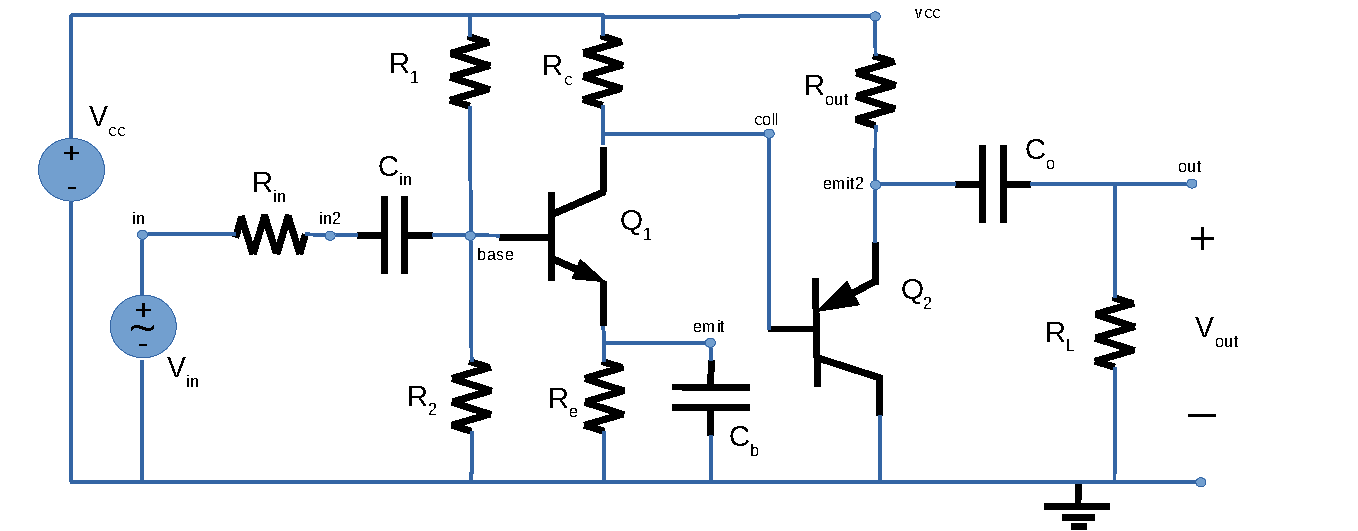
\includegraphics[width=\linewidth]{circuit.pdf}
  \caption{Amplifier circuit}
  \label{fig:theoplots}
  \endminipage\hfill
\end{figure}


The use of an amplifier generally means the ability to obtain an output signal with a greater amplitude in relation to its source signal. An example of using this type of circuit is the simplest microphones that can be found on the market.


